%*----------- SLIDE -------------------------------------------------------------
\begin{frame}[c]{Introdução} 
    \transdissolve[duration=0.5]
   
    \begin{center}
        \Wider{%
        \begin{shaded}
        \begin{center}
            \vspace*{0.5cm}
            \resizebox{!}{0.7cm}{%
                \color{bg} O que é o raspode?
            }%
        \end{center}
        \end{shaded}
        }%
    \end{center}
    
\end{frame}

\begin{frame}[t]{Introdução} 
    \transdissolve[duration=0.5]
    Robô hexapode que tem como objetivo se tornar uma plataforma de aprendizagem para navegação autônoma e cinemática inversa.
    %\newline
        \begin{columns}[t]
            \column{.05\linewidth}
            \column{.5\linewidth}
                \begin{itemize}
                    \item IEEE RAS CIMATEC;
                    \item ROS2 Foxy;
                    \item Navegação autônoma;
                    \item Mapeamento de ambientes.
                \end{itemize}
            \column{.4\linewidth}
            \begin{center}
            %\centerline{
                \begin{figure}
                    \includegraphics[width=0.8\textwidth]{cad.png}
                    \caption{Modelo 3D(Voser, 2021).}
                    % \roundpic[xshift=0cm,yshift=0cm]{2.5cm}{6cm}{pista}
                    %\caption{Pista de corrida \cite{agostini2007}}
                \end{figure}
            %}
            \end{center}
        \end{columns}
%*----------- notes
    \note[item]{Notes can help you to remember important information. Turn on the notes option.}
\end{frame}

\begin{frame}[t]{Objetivos}
    Desenvolver competência em:
    \begin{itemize}
        \item ROS 2 - Foxy;
        \item Cinemática inversa;
        \item Sistemas de controle aplicado a patas de 3 juntas;
        \item Navegação Autônoma utilizando planejadores de trajetória;
        \item Mapeamento 3D de ambientes utilizando visão computacional.
    \end{itemize}
%*----------- notes
    \note[item]{Notes can help you to remember important information. Turn on the notes option.}
\end{frame}

\begin{frame}[t]{Metodologia} 
    \framesubtitle{DIP\&T}
    \transdissolve[duration=0.5]
    \centering
    \begin{figure}
        
        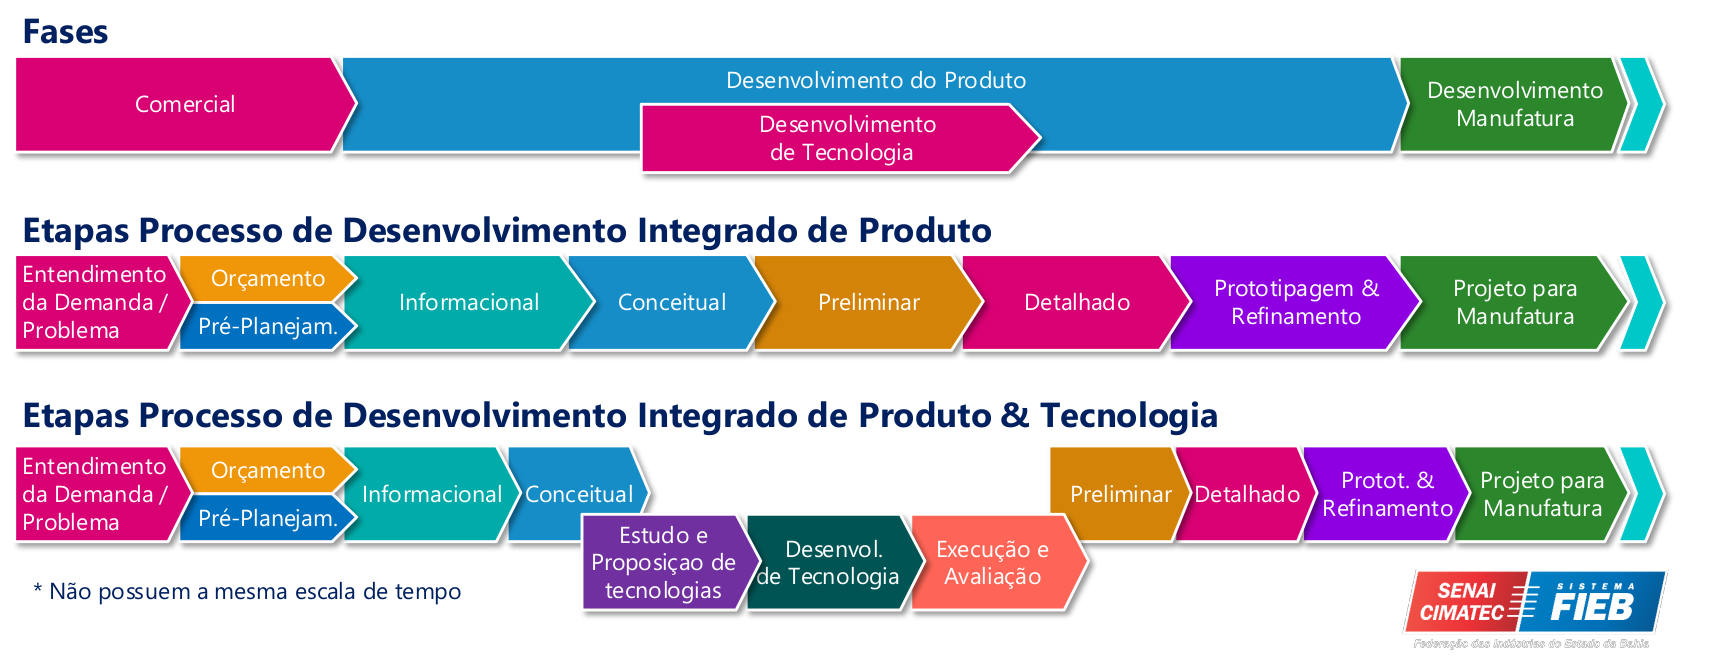
\includegraphics[width=0.8\textwidth]{dipt.png}\\
        \caption{Etapas do Processo utilizando o DIP\&T}
    \end{figure}
    
\end{frame}

\begin{frame}[t]{Metodologia} 
    \framesubtitle{Adaptação do DIP\&T}
    \transdissolve[duration=0.5]
    \centering
    \begin{figure}
        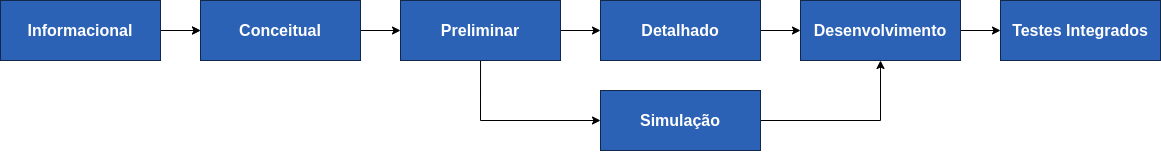
\includegraphics[width=.95\textwidth]{dipt-setps.png}\\
        \caption{Etapas da metodologia.}
    \end{figure}
    
\end{frame}


\begin{frame}[t]{Metodologia} 
    \transdissolve[duration=0.5]
    \centering
    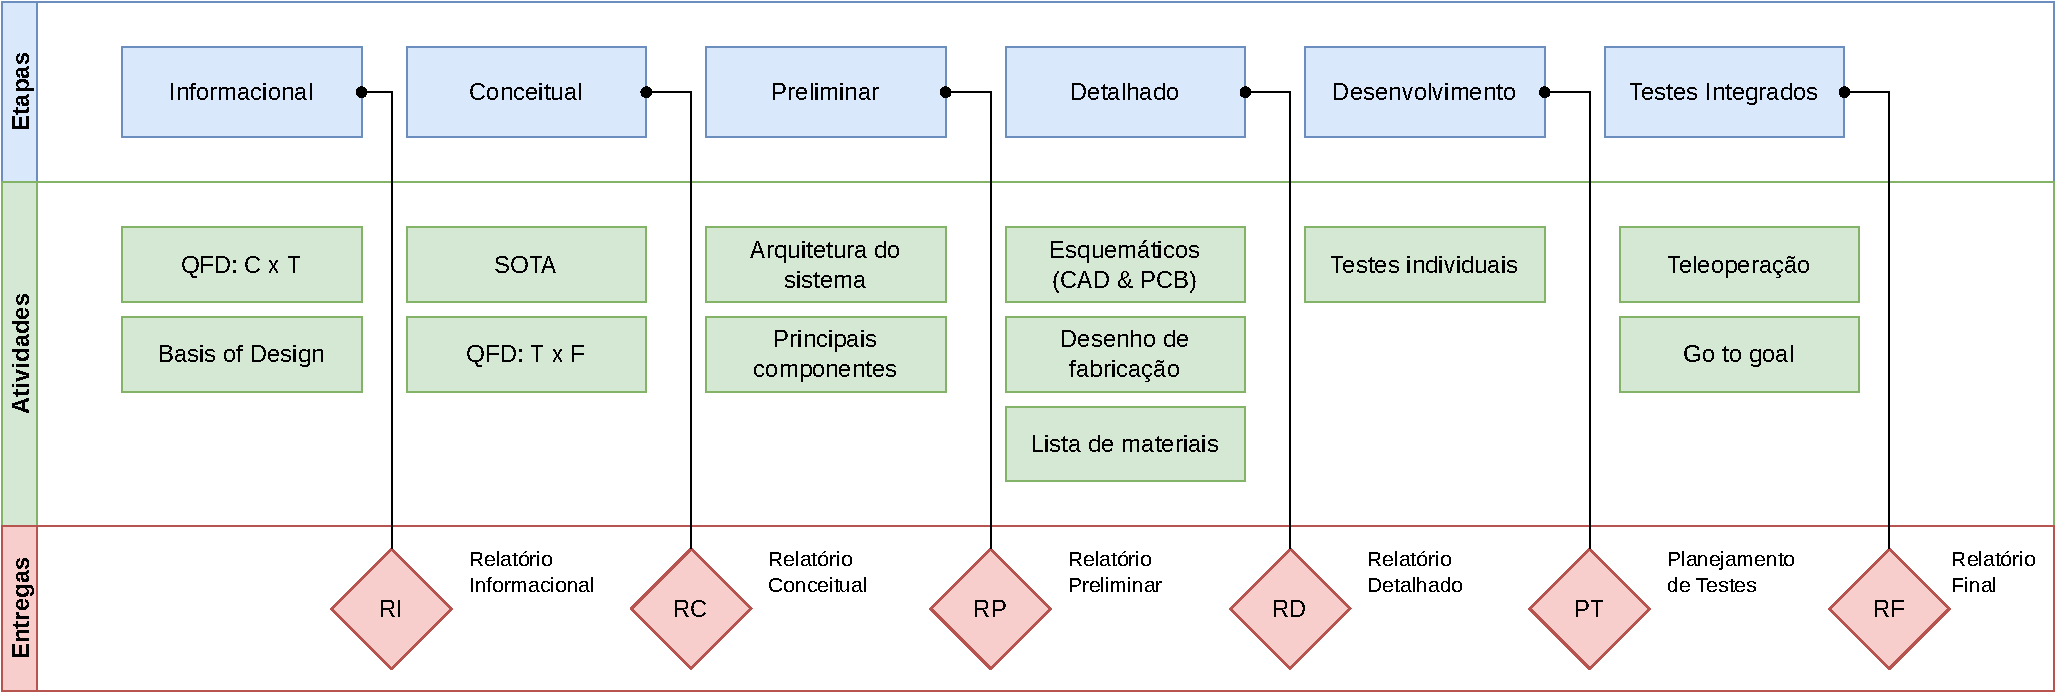
\includegraphics[width=\textwidth]{diagram-4.pdf}
\end{frame}



\begin{frame}[t]{Inspiração}
    \framesubtitle{Leptan project}

    \transdissolve[duration=0.5]
    \centering
    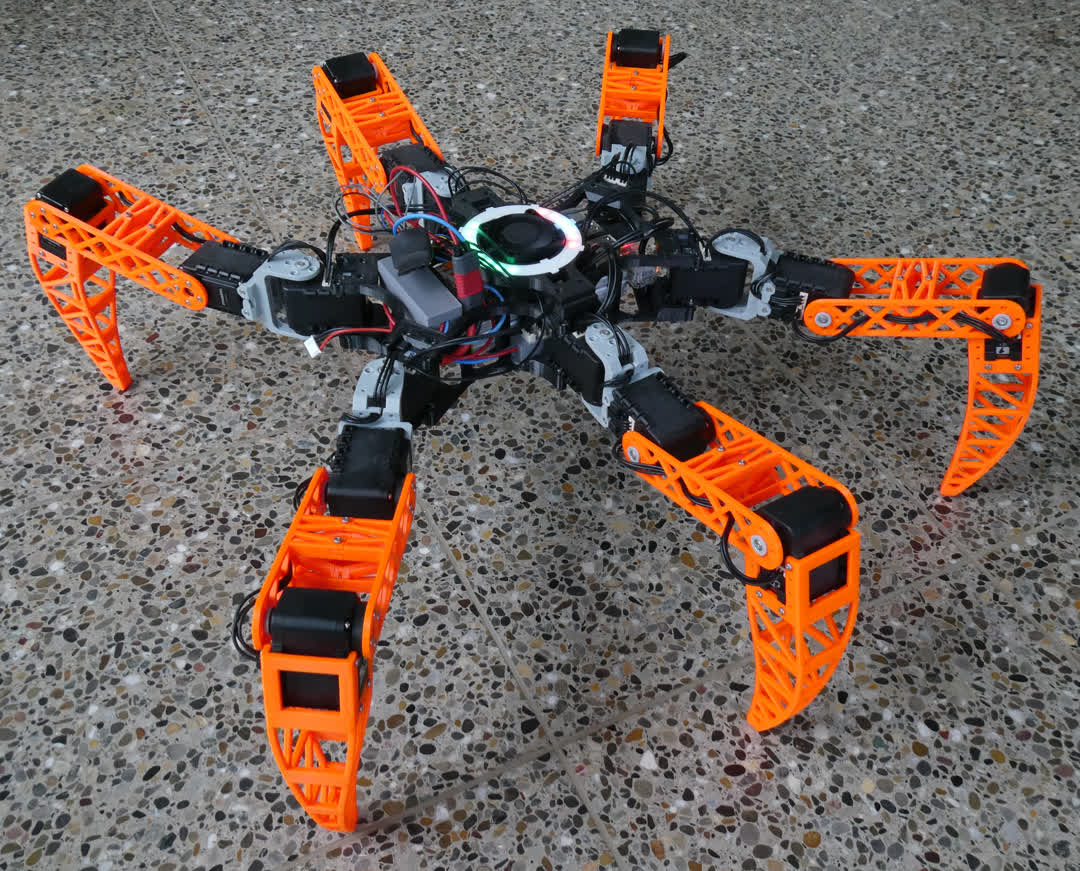
\includegraphics[width=0.5\textwidth]{real.png}

\end{frame}

\begin{frame}[t]{Inspiração}
    \transboxout[duration=0.5]
    \framesubtitle{Leptan project}
    \begin{columns}
        \column{.1\textwidth}
        \column{.4\textwidth}
            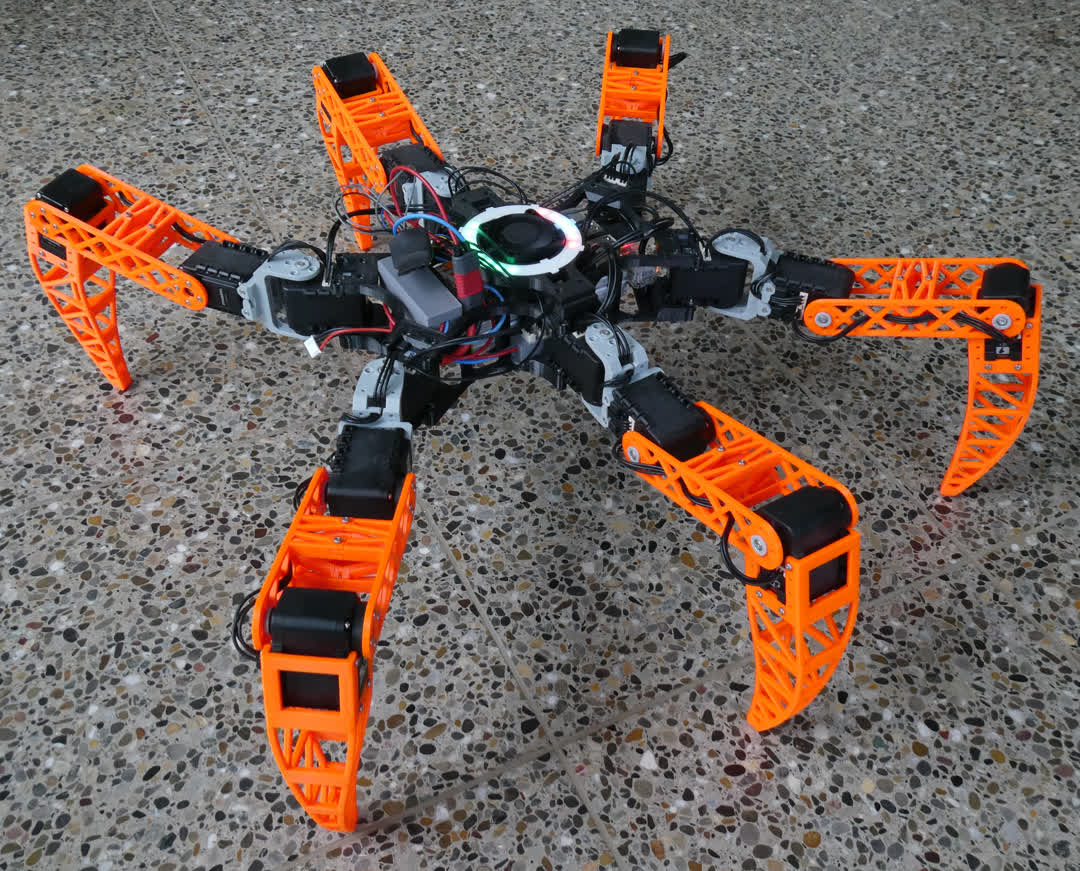
\includegraphics[width=.87\textwidth]{real.png}
        \column{.6\textwidth}
            Através de teleoperação, é possível:
            \begin{itemize}
                \item Levantar e deitar;
                \item Caminhar em qualquer direção;
                \item Girar em torno do seu próprio eixo.
            
            \end{itemize}
    \end{columns}
   
\end{frame}

\begin{frame}[t]{Modelo 3D}

    \transdissolve[duration=0.5]
    \centering
    \includegraphics[width=0.7\textwidth]{cad}

\end{frame}

%*----------- SLIDE -------------------------------------------------------------
\begin{frame}[c]{Simulação}
    \framesubtitle{Estado Atual - Controlado por Teleoperação}
    \begin{center}
    
        \includemedia[
            width=0.7\linewidth,
            totalheight=0.39375\linewidth,
            activate=pageopen,
            passcontext, 
            %transparent,
            addresource=./Source/movies/raspode-movement.mp4,
            flashvars={
            source=./Source/movies/raspode-movement.mp4
            &autoPlay=true
            &autoRewind=true
            &loop=true}
            ]{\fbox{\includegraphics{Source/pictures/cad.png}}}{VPlayer.swf}
    \end{center}

%*----------- notes
    \note[item]{Notes can help you to remember important information. Turn on the notes option.}
 \end{frame}
%-
%*----------- SLIDE -------------------------------------------------------------

\begin{frame}[c]{Materiais}
    \begin{center}
        % Please add the following required packages to your document preamble:
% \usepackage[table,xcdraw]{xcolor}
% If you use beamer only pass "xcolor=table" option, i.e. \documentclass[xcolor=table]{beamer}
\begin{table}[]
    \small
    \begin{tabular}{lll}
    \rowcolor[HTML]{FCFCFC} 
    {\color[HTML]{404040} \textbf{Qty.}} & {\color[HTML]{404040} \textbf{Part name}}                  & {\color[HTML]{404040} \textbf{Description}}  \\
    \rowcolor[HTML]{F3F6F6} 
    {\color[HTML]{404040} 1}             & {\color[HTML]{404040} Raspberry Pi 4}                      & {\color[HTML]{404040} }                      \\
    \rowcolor[HTML]{FCFCFC} 
    {\color[HTML]{404040} 1}             & {\color[HTML]{404040} LiPo 3S}                             & {\color[HTML]{404040} Battery}               \\
    \rowcolor[HTML]{F3F6F6} 
    {\color[HTML]{404040} 1}             & {\color[HTML]{404040} WS2812B LED ring}                    & {\color[HTML]{404040} 24 RGB LEDs}           \\
    \rowcolor[HTML]{FCFCFC} 
    {\color[HTML]{404040} 1}             & {\color[HTML]{404040} 40mm PWM Fan}                        & {\color[HTML]{404040} }                      \\
    \rowcolor[HTML]{F3F6F6} 
    {\color[HTML]{404040} 1}             & {\color[HTML]{404040} Adafruit INA260}                     & {\color[HTML]{404040} Voltage/Current meter} \\
    \rowcolor[HTML]{FCFCFC} 
    {\color[HTML]{404040} 18}            & {\color[HTML]{404040} Dynamixel AX-12A}                    & {\color[HTML]{404040} Servo}                 \\
    \rowcolor[HTML]{F3F6F6} 
    {\color[HTML]{404040} 1}             & {\color[HTML]{404040} Dynamixel U2D2}                      & {\color[HTML]{404040} Servo Interface}       \\
    \rowcolor[HTML]{FCFCFC} 
    {\color[HTML]{404040} 1}             & {\color[HTML]{404040} ROBOTIS Robot Cable-3P 140mm 10 pcs} & {\color[HTML]{404040} Cable}                 \\
    \rowcolor[HTML]{F3F6F6} 
    {\color[HTML]{404040} 1}             & {\color[HTML]{404040} ROBOTIS Robot Cable-3P 180mm 10 pcs} & {\color[HTML]{404040} Cable}                 \\
    \rowcolor[HTML]{FCFCFC} 
    {\color[HTML]{404040} 1}             & {\color[HTML]{404040} ROBOTIS Robot Cable-3P 200mm 10 pcs} & {\color[HTML]{404040} Cable}                 \\
    \rowcolor[HTML]{F3F6F6} 
    {\color[HTML]{404040} 1}             & {\color[HTML]{404040} ROBOTIS P04-F2 10pcs}                & {\color[HTML]{404040} }                      \\
    \rowcolor[HTML]{FCFCFC} 
    {\color[HTML]{404040} 1}             & {\color[HTML]{404040} ROBOTIS P04-F3 10pcs}                & {\color[HTML]{404040} }                      \\
    \rowcolor[HTML]{F3F6F6} 
    {\color[HTML]{404040} 2}             & {\color[HTML]{404040} ROBOTIS BPF-WA/BU 10pcs}             & {\color[HTML]{404040} }                      \\
    \rowcolor[HTML]{FCFCFC} 
    {\color[HTML]{404040} 10}            & {\color[HTML]{404040} MOLEX 22-03-5035}                    & {\color[HTML]{404040} PCB Connectors}       
    \end{tabular}
    \end{table}
   \end{center}

%*----------- notes
    \note[item]{Notes can help you to remember important information. Turn on the notes option.}
 \end{frame}
